%----------------------------------------------------------------------------
\chapter{Tervezés és megvalósítás}
%----------------------------------------------------------------------------

A rendszer architektúrájának tervezése során figyelembe vettem a \ref{research}. és \ref{scopes}. fejezetekben kitűzött célokat. Az eretedi tervek elkészültével kezdetét vette a megvalósítás. Az implementáció során felmerültek olyan akadályok és újabb ötletek, amelyek kisebb-nagyobb mértékben befolyásolták a terveket. Erre számítottam és éppen ezért úgy próbáltam tervezni, hogy dinamikusan módosíthatóak legyenek és bővítés vagy módosítás esetén. A tervezési és megvalósítási folyamat hónapokat vedd igénybe annak érdekében, hogy minden jelentkező problémát és az újabb ötleteket legyen idő átgondolni.

\section {Az alkalmazás frontendje}

\subsection {Kezdőoldal (Homepage)}

Tekintettel arra, hogy az alkalmazás bizonyos funkcionalitásai használhatóak bejelentkezés nélkül is, a kezdőoldal egy üdvözlő oldal egy navigációs menüvel az oldal tetején. Amennyiben egy eszközről első alkalommal lépik az oldalra egy felhasználó, akkor egy információs ablakkal találkozik, amely tartalmazza az alkalmazás célját, a hivatalos forrásokat a jegyvásárlásra és ezeknek a jogtulajdonosait (\ref{abra:homepagePopup}).

Annak érdekében, hogy ez az ablak csak egyszer jelenleg meg \textbf{sütiket (Cookies)} használok. Ezek a sütiket a böngésző tárolja a felhasználó eszközén és a weboldal betöltésekor a böngésző betölti az elmentett sütiket, ha vannak. Ezek kulcs-elem párok, amely értelmében egy tetszőleges nevű kulcs alatt tudok elmenteni majdnem bármilyen adatot. Ha a felhasználó rákattint az \textbf{Understood} gombra, akkor egy \textbf{modalAccepted} kulcs alatti sütiben eltárolom a \textbf{true} értéket és amikor betöltődik az alkalmazás ezt az értéket ellenőrzöm.
Mint említettem ezek a sütik lokálisan vannak tárolva a felhasználónál és ha a felhasználó kitörli azokat, amelyek ehhez az oldalhoz tartoznak, akkor egyértelműen újra elő fog jönni egy az ablak.

\begin{figure}[!h]
	\centering
	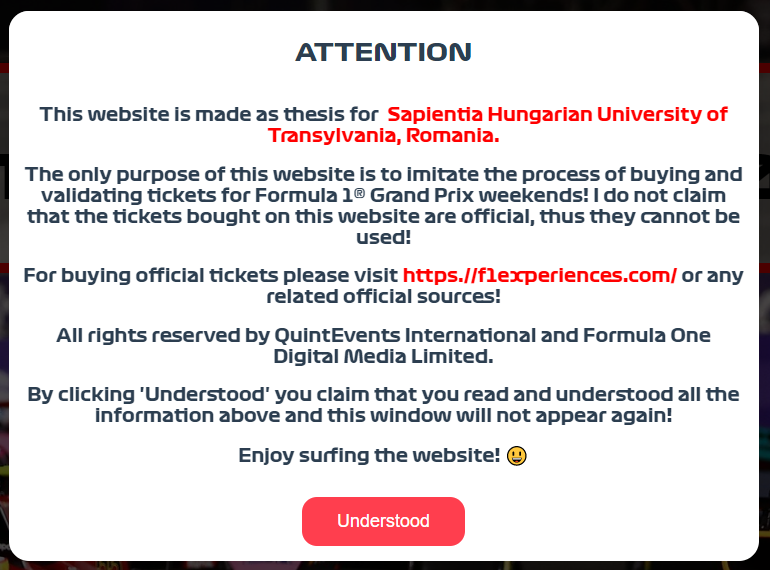
\includegraphics[scale=0.4]{images/homepagePopup}
	\caption{Kezdőoldalon felugró ablak}
	\label{abra:homepagePopup}
\end{figure}
\pagebreak

\begin{figure}[!h]
	\centering
	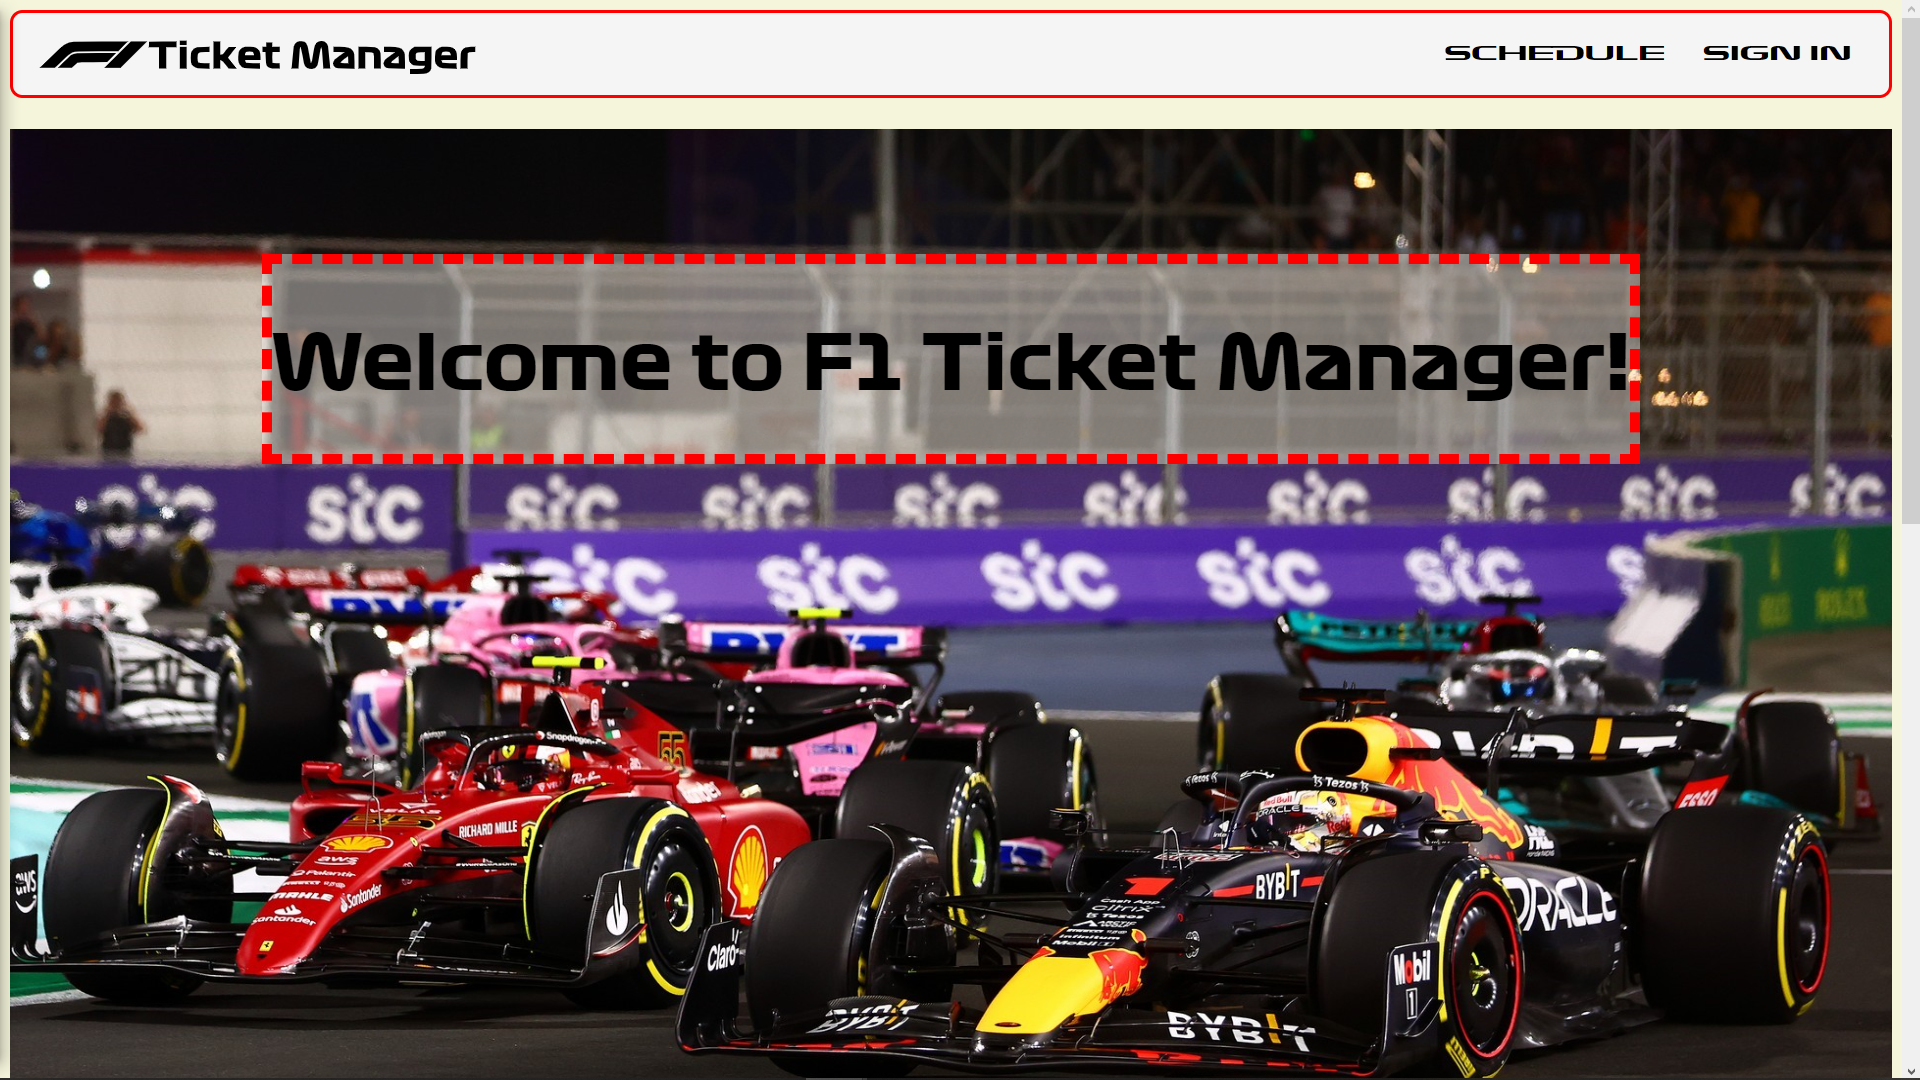
\includegraphics[scale=0.2]{images/homepage}
	\caption{Kezdőoldal}
	\label{abra:homepage}
\end{figure}
\pagebreak

\subsection {Versenynaptár (Schedule)}

A \textbf{Versenynaptár} oldalon lehet böngészni a 2022-es év versenyeinek listáját a megrendezési sorrendben. Az első kártya, ami megjelenik az oldalon az a következő verseny, amely automatikusan kerül ki az aktuális dátum alapján. Teszt jelleggel van egy dátum kiválasztó gomb is, hogy ki lehessen próbálni, hogy egy adott dátumhoz melyik verseny lesz a legközelebb. Erre a kártyára kattintva meg lehet tekinteni a részleteket. Minden kártyán látszanak a legfontosabb információk az adott versenyről, mint a pálya neve, a rendező ország neve, az intervallum, amikor az esemény zajlani fog és a pályarajz (\ref{abra:schedule}).

\begin{figure}[!h]
	\centering
	\begin{tabular}{cc}
	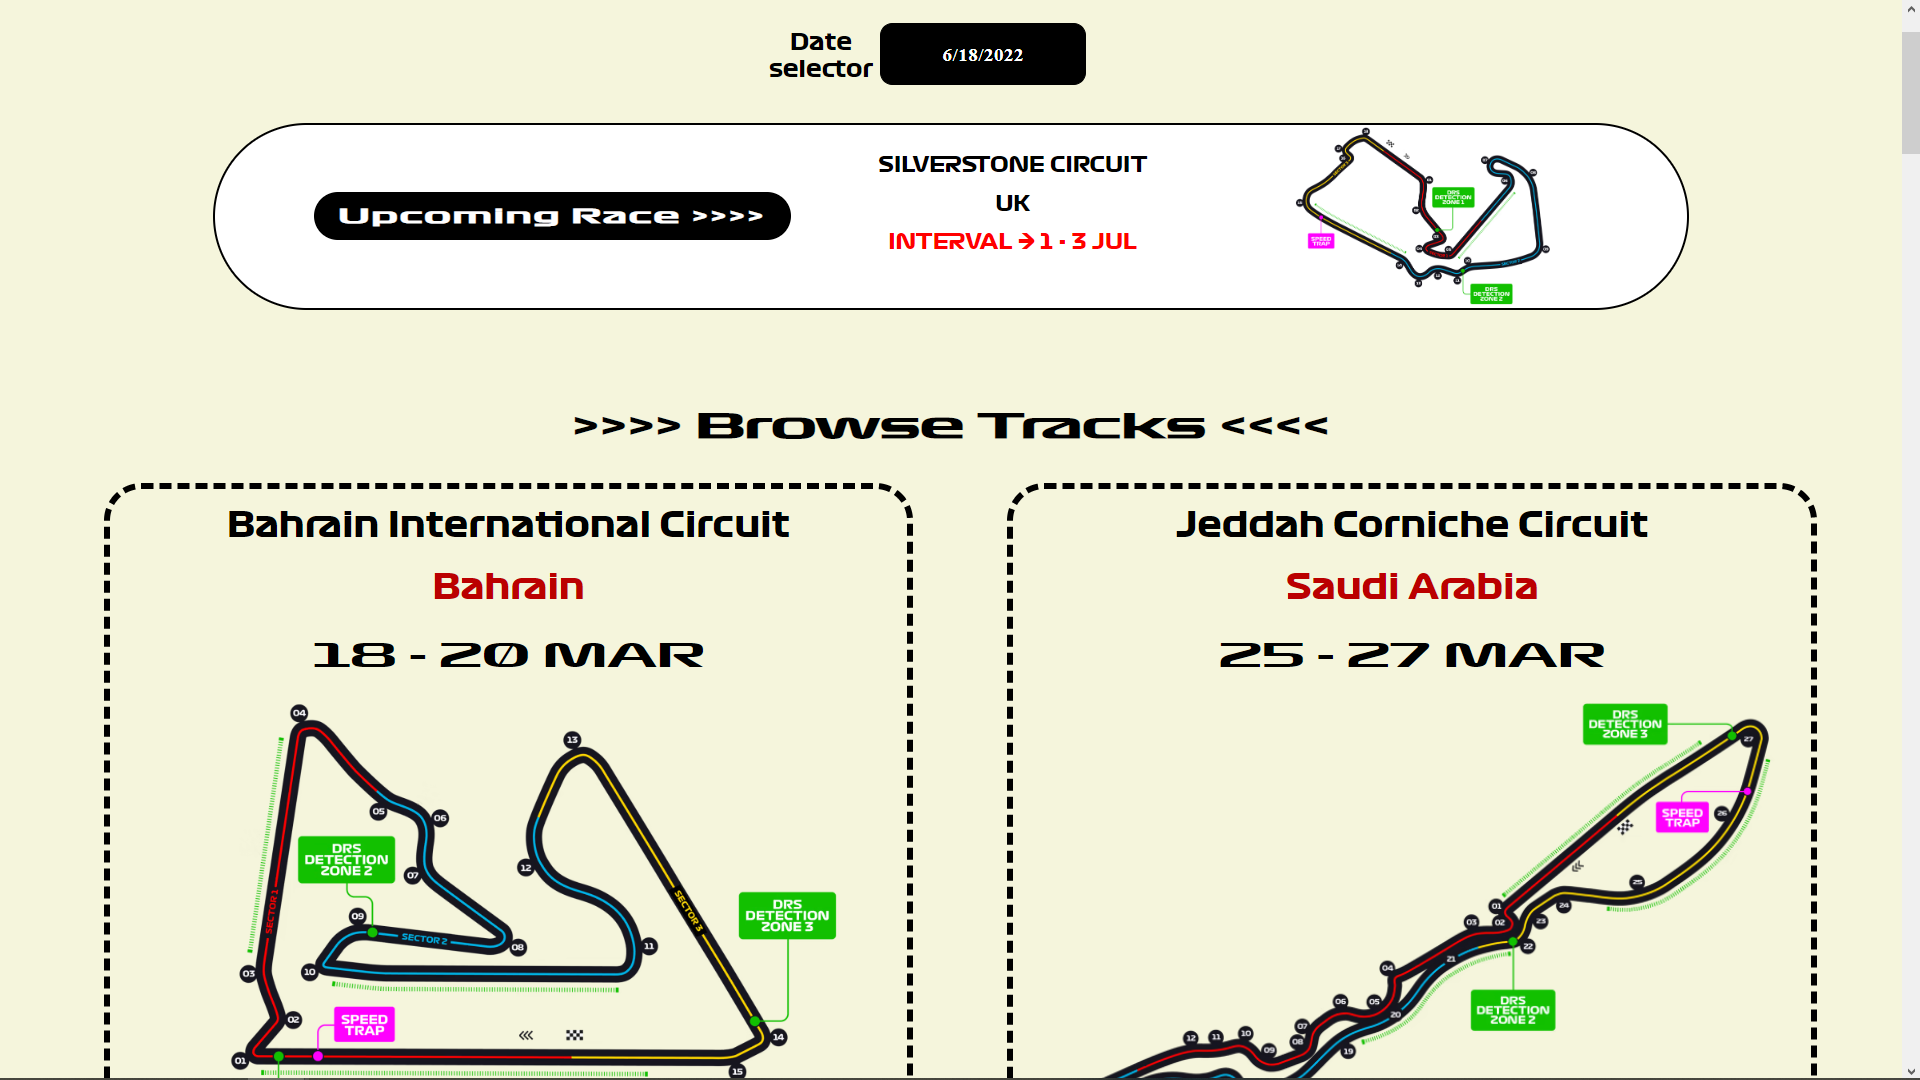
\includegraphics[scale=0.15]{images/schedule1} &
	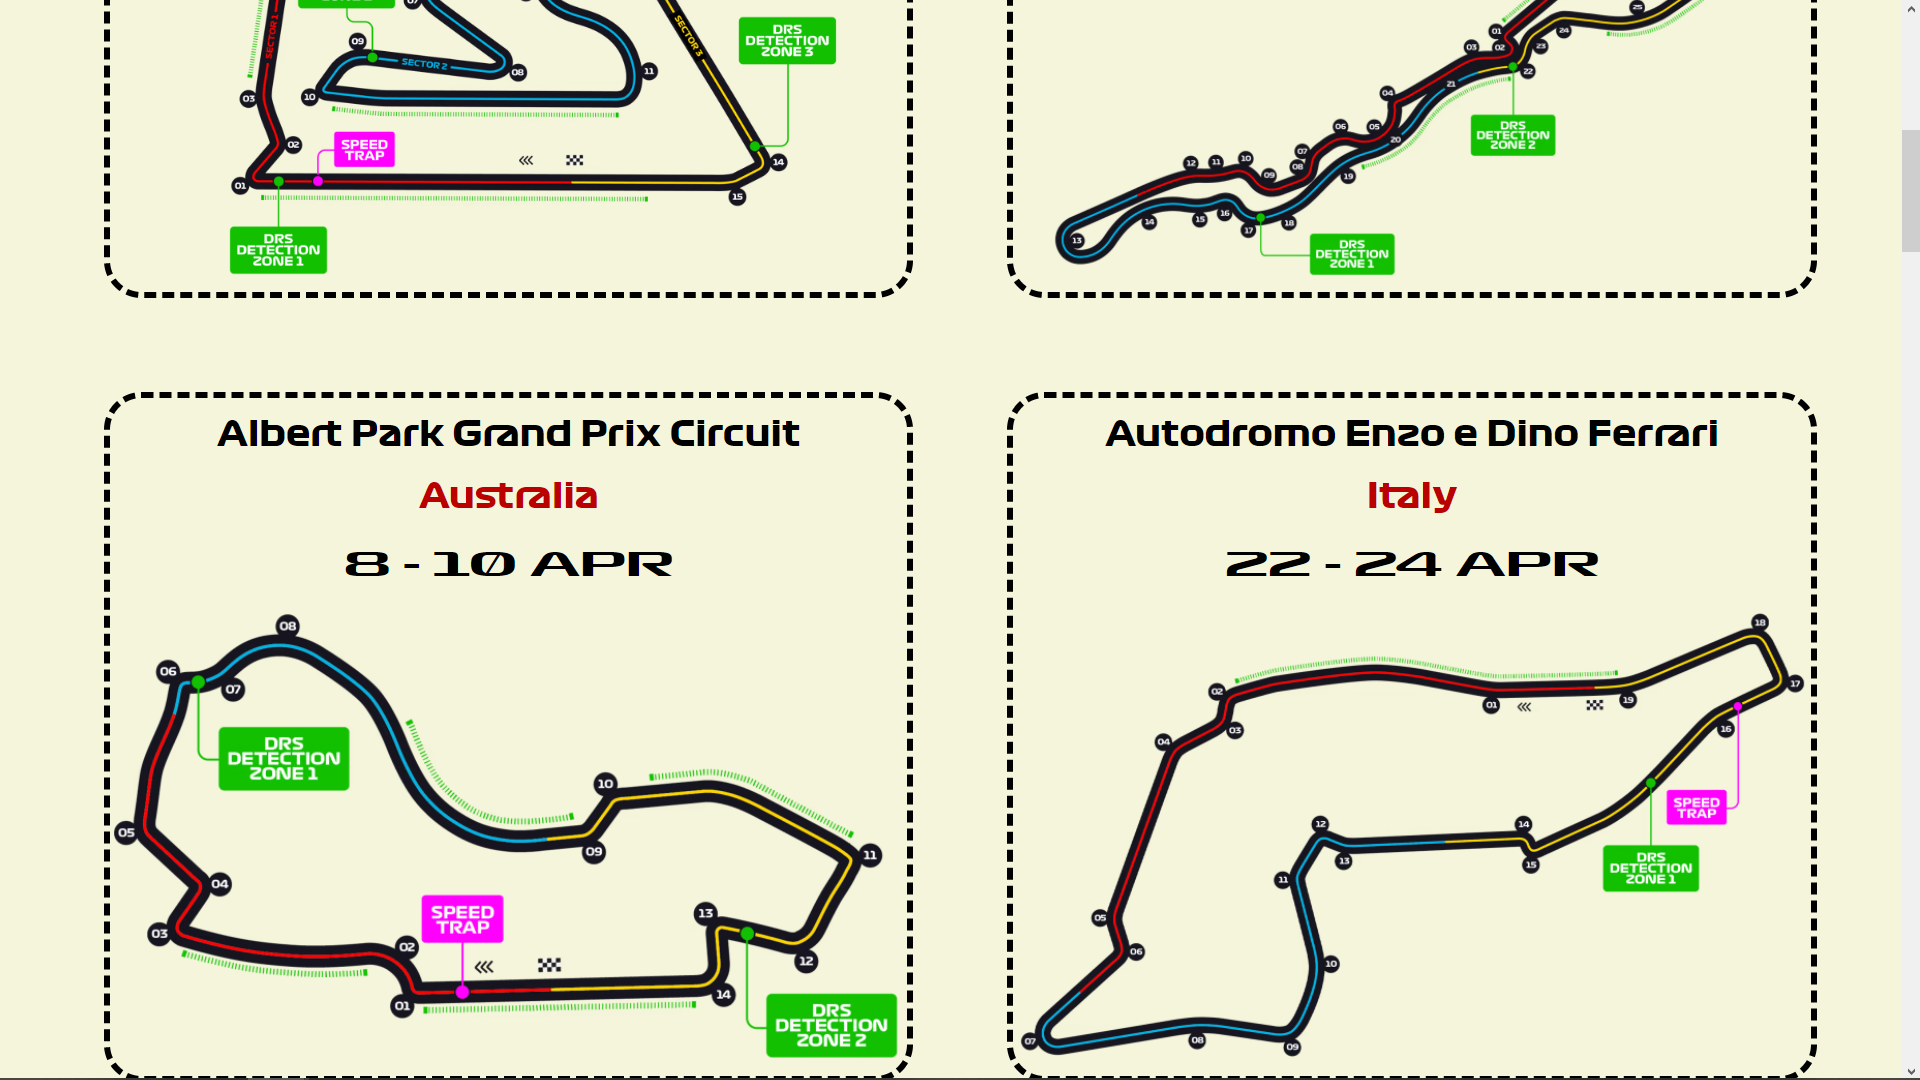
\includegraphics[scale=0.15]{images/schedule2} \\
	A versenynaptár & Görgetéssel látható az összes pálya
	\end{tabular}
	\caption{Versenynaptár}
	\label{abra:schedule}
\end{figure}

Ha átvisszük az egeret a kártya fölott, akkor mgejelenik egy gomb \textbf{Browse tickets} szöveggel, amelyre kattintva megtekinthetőek a versenyhez tartozó jegy típusok és azok információi (\ref{abra:ticketsUA}). Ha nincs bejelentkezve a felhasználó, akkor az \textbf{Add to cart} gomb szürkén jelenik meg, vagyis nem lehet a kosárba tenni, viszont ha rákattint a felhasználó, akkor a rendszer jelezni fogja egy \textbf{alert} (figyelmeztetés) ablakban, hogy autentikáció szükséges, ha ezt a funkciót szeretné használni.

\begin{figure}[!h]
	\centering
	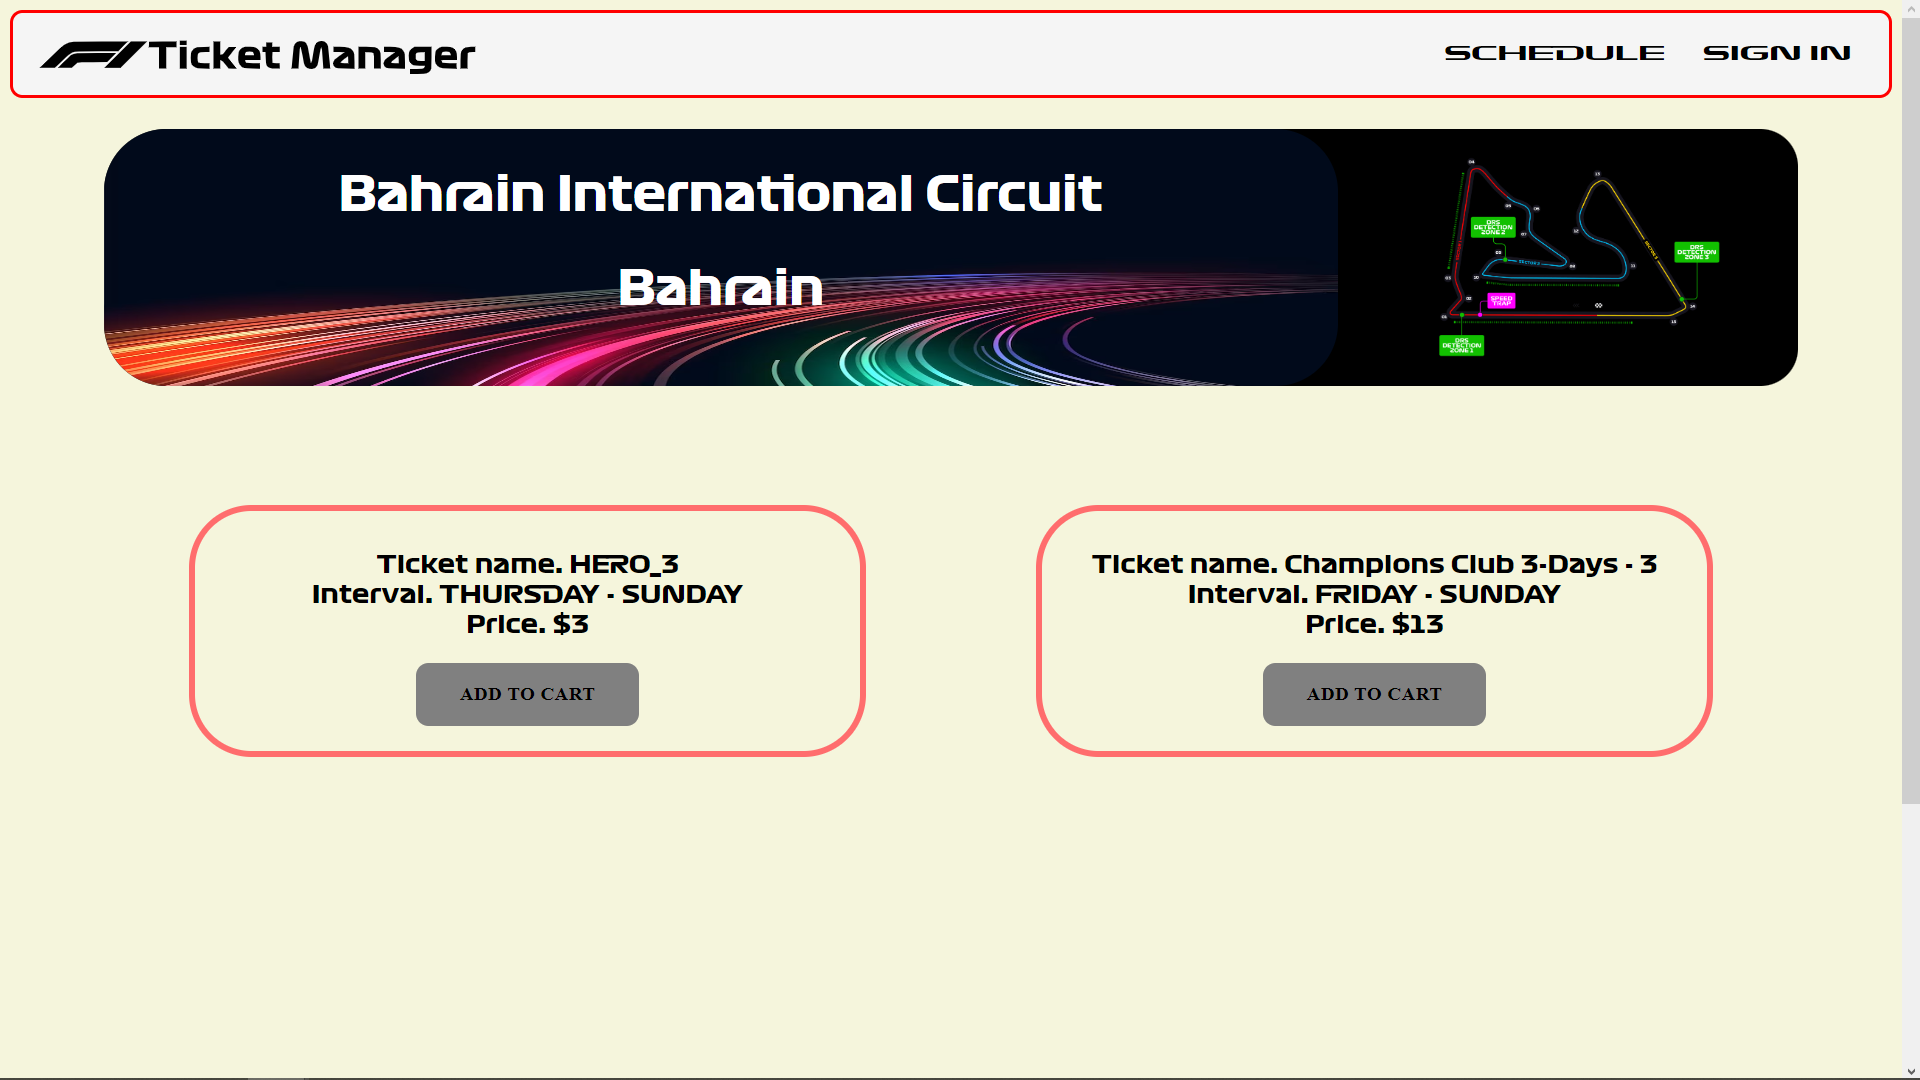
\includegraphics[scale=0.2]{images/tickets}
	\caption{Jegy típusok be nem jelentkezett felhasználóval}
	\label{abra:ticketsUA}
\end{figure}

Abban az esetben, ha a felhasználó be van jelentkezve, lehetőség van a jegyet a kosárba helyezni vagy visszajelzést adni az adott jegyről, élményekről (\ref{abra:ticketsAuth}). A jegyek mennyiségét a \textbf{Checkout} oldalon van lehetősége módosítani a felhasználónak. A rendszer ezen része egy továbbfejlesztési terület, hogy adott esetben ellenőrizve legyen, hogy tényleg csak az tudjon visszajelzést adni, akkor vásárolt az adott jegyből. 

\begin{figure}[!h]
	\centering
	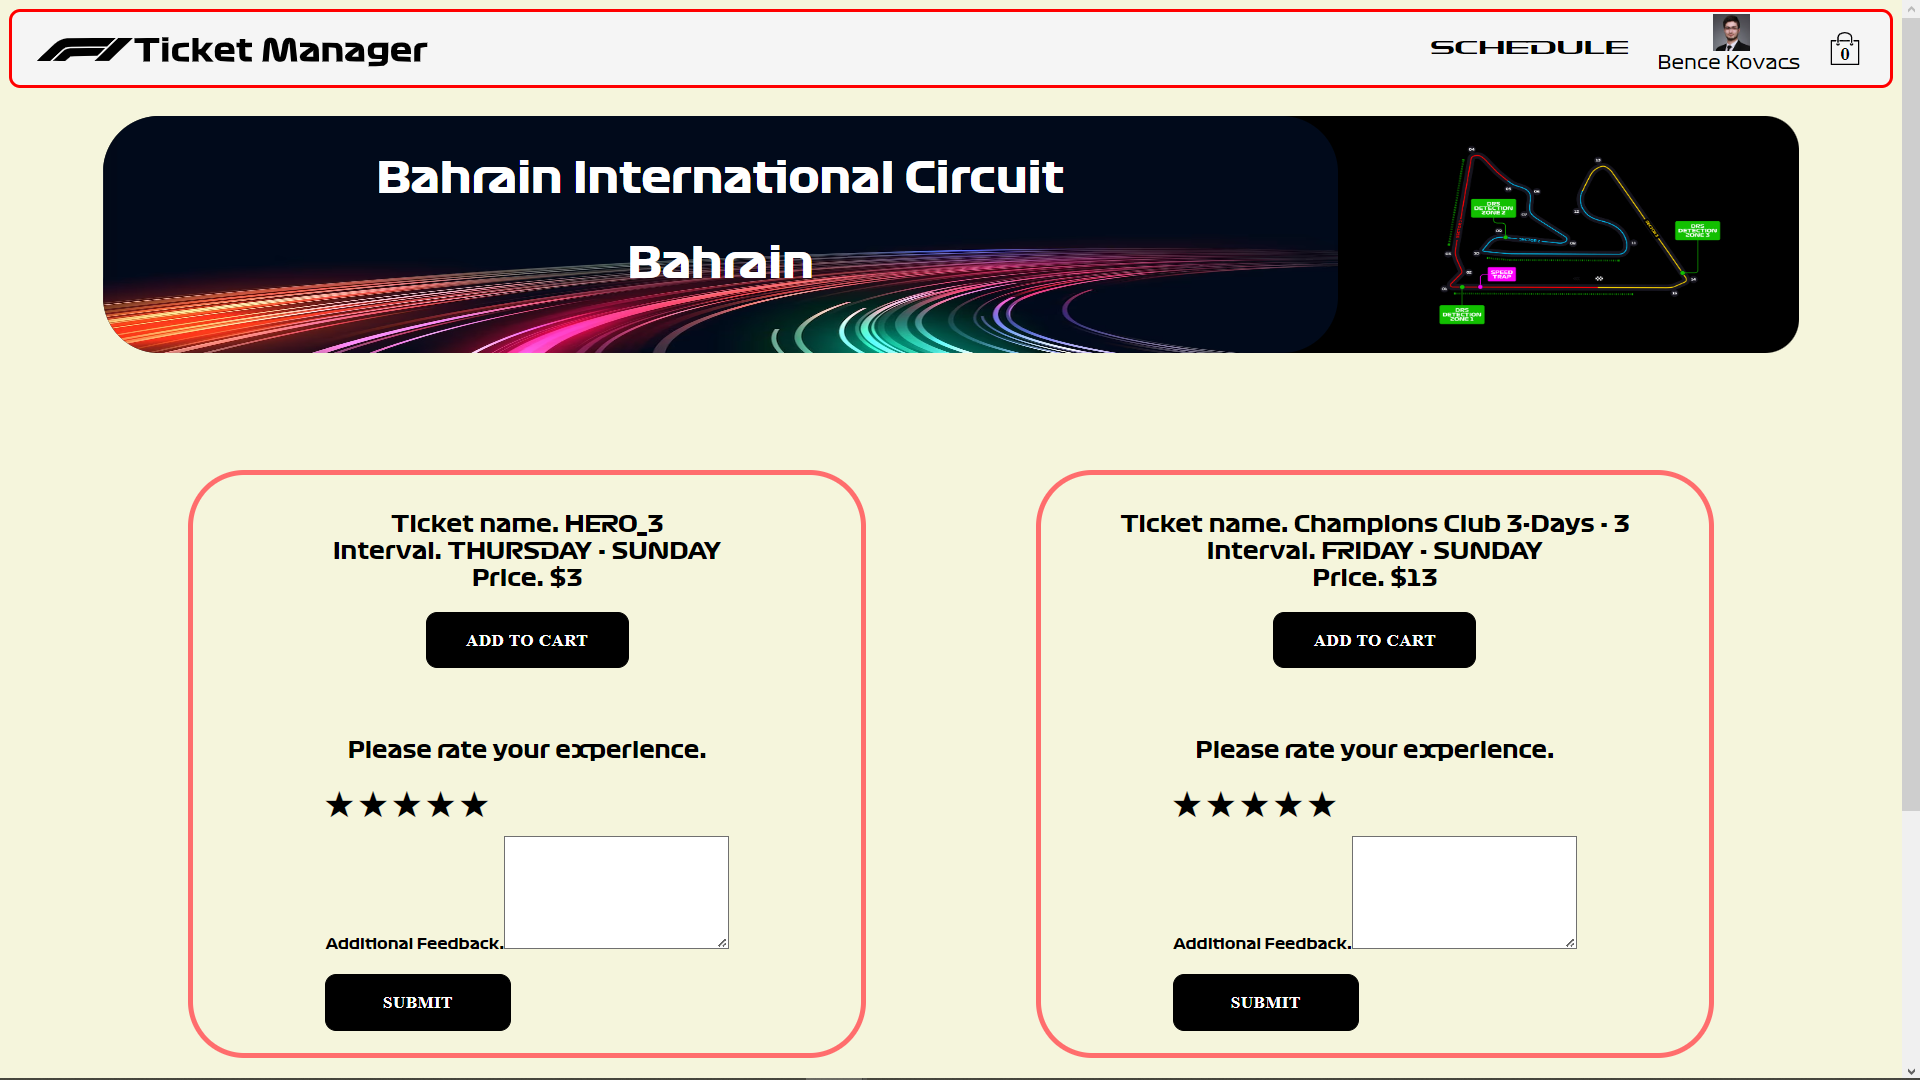
\includegraphics[scale=0.2]{images/ticketsAuth}
	\caption{Jegy típusok bejelenkezett felhasználóval}
	\label{abra:ticketsAuth}
\end{figure}

\subsection {Profil (Profile)}

A \textbf{Profil} oldal elérése csak a bejelentkezett felhasználóval lehetséges (\ref{abra:profile}). Ezen az oldalon lehetséges a profilkép és a megjelenített név módosítása az \textbf{Edit profile} gombra kattintva.

\begin{figure}[!h]
	\centering
	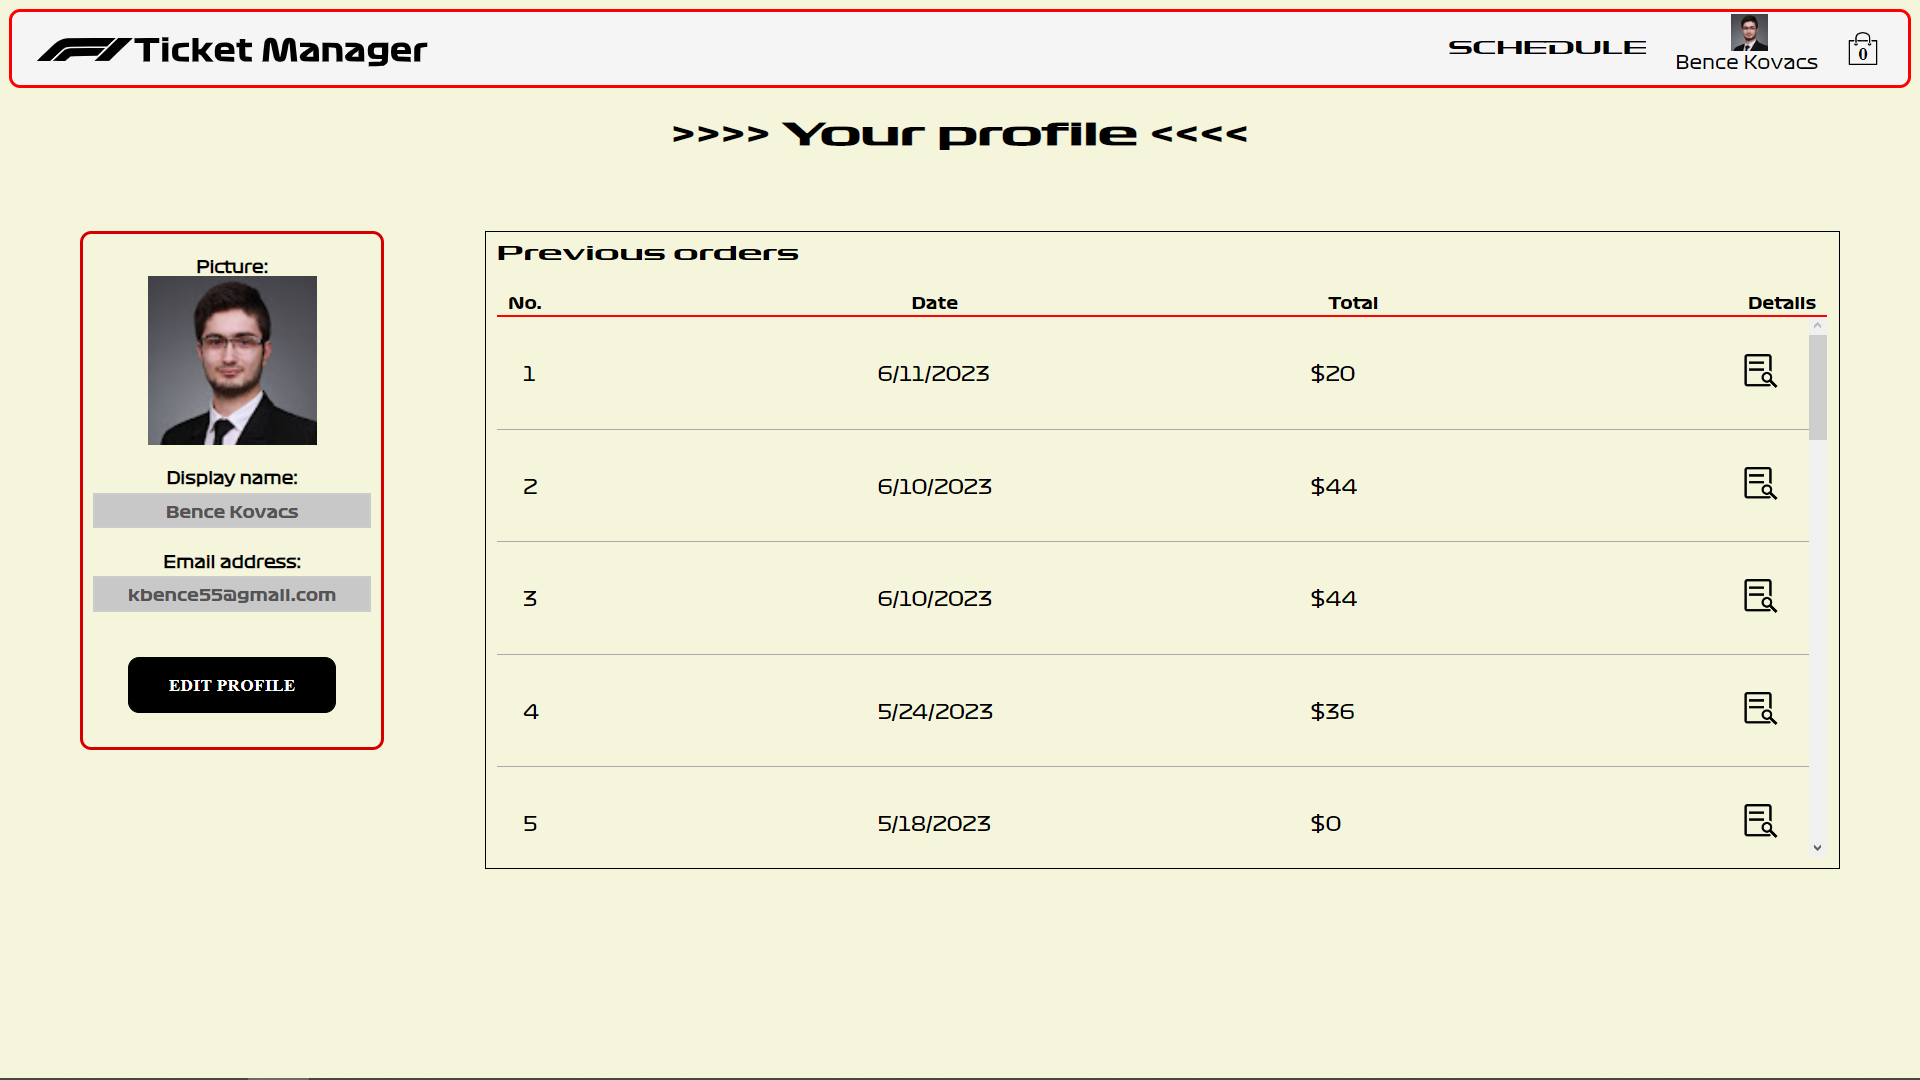
\includegraphics[scale=0.2]{images/profile}
	\caption{Saját profil oldal}
	\label{abra:profile}
\end{figure}

Az oldal jobb részén láthatóak a \textbf{rendelési előzmények}. Ezek görgetéssel böngészhetőek és a jobb szélén levő ikonra kattintva tekinthetőek meg a vásárlás részletei (\ref{abra:previousOrders}).

\begin{figure}[!h]
	\centering
	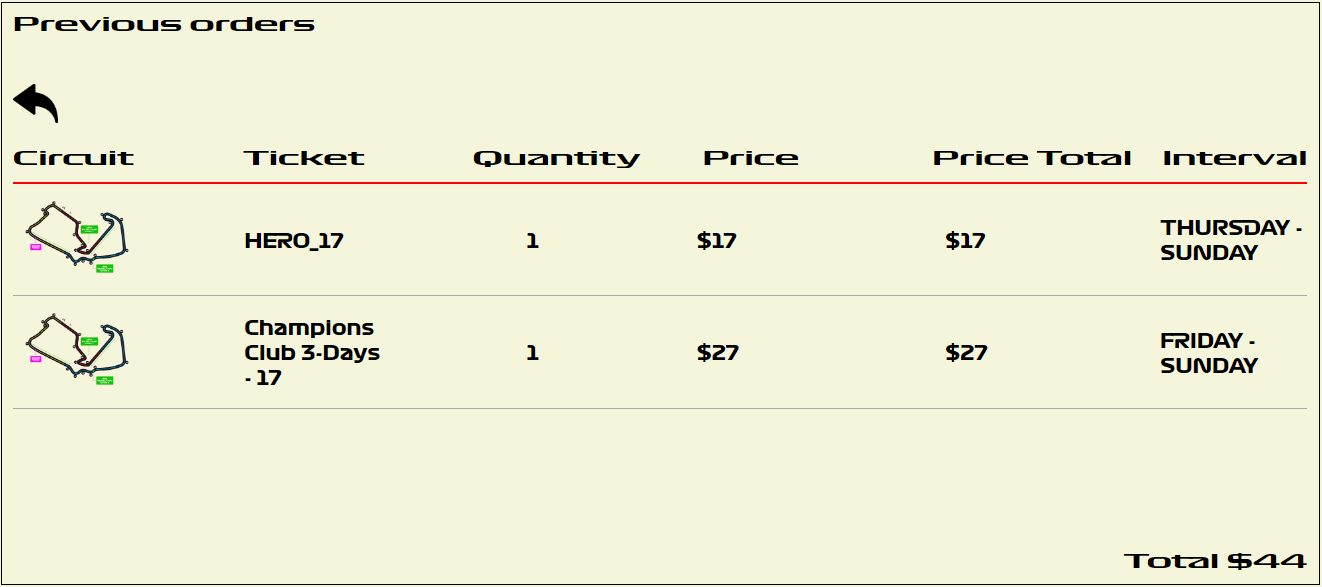
\includegraphics[scale=0.3]{images/previousOrders}
	\caption{Rendelés részletei}
	\label{abra:previousOrders}
\end{figure}

Amennyiben elvisszük valamely elem fölött az egeret megjelenik egy \textbf{More details} gomb, amelyre kattintva megtekinthető a jegy egyedi azonosítója (\ref{abra:moreDetails}). Ez a funkcionalitás azért fontos, mivel megtörténhet, hogy a felhasználó elveszíti vagy nem kapja meg a QR kódot emailben, ami ezt az azonosítót tartalmazza. Ha ez bekövetkezne, akkor innen is lehetőség van kimásolni és a megszokott módon azonosítani a PIN kóddal.

Ezen a felugró ablakon továbbá lehetősége van a felhasználónak egy új PIN kódot megadni, ha a meglévő elfelejtette vagy úgy érzni, hogy valaki megszerezhette. Ezután egy újabb felugró ablakban lehetséges a PIN kód megváltoztatása. 

\begin{figure}[!h]
	\centering
	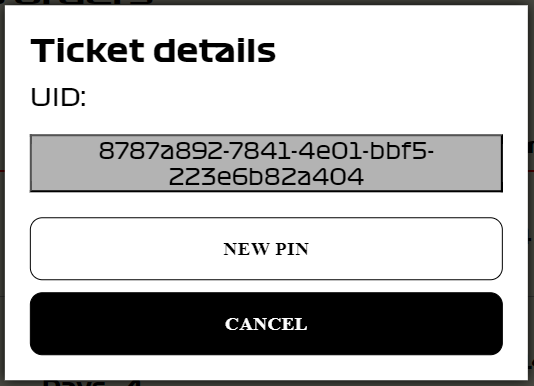
\includegraphics[scale=0.4]{images/moreDetails}
	\caption{Jegy részletei}
	\label{abra:moreDetails}
\end{figure}

A PIN kód megadásánál kötelezően egy 6 számjegyű számot kell megadni (\ref{abra:pinPopup}). Ezt manuálisan is be lehet írni vagy a \textit{pálca} ikonra kattintva generálódik egy véletlenszerű szám. A \textbf{Submit} gombra kattintva frissítheti a felhasználó a jegyhez tartozó kódot, ami teljes mértékben felülírja az előzőt, ezért nagyon figyelmes kell lenni a megadásakor, de erre a pirossal írt szöveg is figyelmezteti a vásárlót.

\begin{figure}[!h]
	\centering
	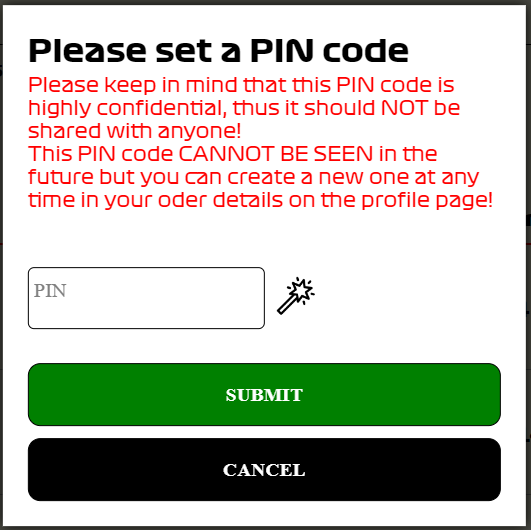
\includegraphics[scale=0.4]{images/pinPopup}
	\caption{PIN kód változtatás ablak}
	\label{abra:pinPopup}
\end{figure}

\pagebreak




////////-------------------------- PROGRESS --------------------------////////

\textbf{Matlab ode45 előnyei:}
\begin{itemize}
	\item nagyon egyszerű a használata, nem igényel komoly programozási ismereteket
	\item könnyű beépíteni és összekötni más Matlab programokkal
	\item a kapott eredményeket mátrix vagy vektor típusokban téríti vissza, ami könnyűvé teszi az eredmények további kezelését
	\item az eredményeket grafikus felületen azonnal meg tudjuk jeleníteni
	\item jobb eredményeket produkált, mint az Odeint
	\item jól dokumentált, sok példa van a használatára
\end{itemize}
\pagebreak
\textbf{Matlab ode45 hátrányai:}
\begin{itemize}
	\item komoly hátránya az Odeinttel szemben, hogy \textbf{fizetni kell a használatáért}
	\item nagyon sok memóriát használ, komolyan igénybeveszi a számítógép erőforrásait
\end{itemize}
\textbf{Odeint előnyei:}
\begin{itemize}
	\item ingyenes és nyílt forráskódú, használható személyi és kereskedelmi célokra egyaránt
	\item nagyon rugalmas, absztrak, így könnyedén változtatható a bemeneti adatok típusa vagy struktúrája 
	\item C++ nyelven írodott, támogatva a modern programozási technológiákat (Generikus programozás, Template Metaprogramming)
\end{itemize}
\textbf{Odeint hátrányai:}
\begin{itemize}
	\item használata nehezebb, mint a Matlab ode45 programé, szükséges a C++ programozási nyelv ismerete
	\item a kapott eredményekkel nem olyan könnyű bánni, mint a Matlab esetében
	\item absztraktsága miatt nehéz a felmerülő problémákat megoldani
	\item dokumentáltsága jóval szegényesebb, mint a Matlabé
\end{itemize}




\begin{figure}
	\centering
	\begin{tikzpicture}
		\node[main node] (1) {$1$};
		\node[main node] (2) [below left = 2.3cm and 1.5cm of 1]  {$2$};
		\node[main node] (3) [below right = 2.3cm and 1.5cm of 1] {$3$};
		
		\path[draw,thick]
		(1) edge node {} (2)
		(2) edge node {} (3)
		(3) edge node {} (1);
		%%
		\begin{scope}[xshift=4cm]
			\node[main node] (1) {$1$};
			\node[main node] (2) [right = 2cm  of 1]  {$2$};
			\node[main node] (3) [below = 2cm  of 1] {$3$};
			\node[main node] (4) [right = 2cm  of 3] {$4$};
			
			\path[draw,thick]
			(1) edge node {} (2)
			(1) edge node {} (4)
			(3) edge node {} (2)
			(3) edge node {} (4)
			;
		\end{scope}
	\end{tikzpicture}
\caption{Egyszer\H u gr\'af TIKZ seg\'its\'eg\'evel}
\end{figure}



\newpage
\section {Saját szoftverek esetén}

Saját szoftverek esetében sikerült négy különböző technológia segítségével megvalósítani a Dorman-Prince differenciálegyenlet megoldó algoritmust (lásd \ref{fejezet3_2}. alfejezet). A felhasznált technológiák: Matlab, Java, C++ és Android voltak.

Ezen technológiák közül az Androidos szoftverrel kapcsolatban már előzetes félelmeink voltak, mivel azt feltételeztük, hogy bármennyire is fejlettek napjainkban a mobileszközök, mégis hardveresen nem lesznek elegek ahhoz, hogy versenybe tudjanak szállni a számítógépekkel. Néhány teszt után feltételezéseink beigazolódtak, láthatjuk a \ref{fejezet3_3}. alfejezet teszteseteiben is, hogy az Android szoftver mennyire gyengén teljesített (mind a Motorola Moto E2, mind a Samsung Galaxy Core Prime esetében). Összehasonlítva a többi algoritmussal az átlagidőket nézve $ 150-160 $ - szor lassabb a Javanál és $ 300 - 350 $ - szer a C++ - nál! Tehát azt a következtetést vonhatjuk le, hogy nem érdemes mobileszközökön differenciálegyenleteket oldani, mivel túlságosan nagy a hardver igénye és egyelőre ezen a téren nem képesek tartani a lépést a számítógépekkel.

A további három technológia közül (Matlab, Java, C++) meglepő módon itt is a Matlab teljesített a legjobban, igaz, hogy ebben az esetben már nem használtuk az ode45 programot, hanem megírtam én a saját függvényemet. Ez a teljesítményen is meglátszott, mert az általam írt függvény nem tudott jobban teljesíteni a tesztek alatt, mint az ode45. Mindezek ellenére $ 35-40 $ - szer gyorsabb volt a Javanál és megközelítőleg $ 15-20 $ - szor gyorsabb a C++ - nál.

A Java és C++ szoftvereket összehasonlítva elmondhatom, hogy az esetek többségében a C++ körülbelül $ 2 $ - szer volt gyorsabb a Javanál, ami megfelel az előzetes elvárásoknak.

Amit nagyon fontosnak tartok kihangsúlyozni, hogy az általam megvalósított C++ szoftver a tesztek során nagyon jól teljesített, felvette a versenyt az Odeint könyvtárral és az elért átlagok is csak nagyon kicsivel maradnak el az Odeint által produkált eredményektől (\ref{fejezet3_3}. alfejezet).

Továbbá megvalósítottam az Euler és Runge-Kutta módszerek párhuzamosított változatait is CUDA technológia segítségével. Ebben az esetben a tesztek azt mutatták, hogy az Euler módszer esetében többe kerül a sok CPU és GPU memória közötti másolás művelete, mint amennyit nyerünk a számítások elvégzése során. Tehát ebben az esetben ez a fajta párhuzamosítási megközelítés nem éri meg. Ezzel ellentétben a Runge-Kutta módszer esetében a megközelítés eredményesnek bizonyult abban az esetben, ha az egyenletek száma nagy és a lépésköz kicsi. A \ref{fejezet3_4} alfejezetben láthattuk, hogy abban az esetben ha az egyenletek száma $ n = 10 $ és a lépésköz $ h = 0.001 $, a GPU-n megközelítőleg 5 és fél perccel hamarabb lefutott az algoritmus, mint a CPU-n. Ezzel a párhuzamosítási módszerrel nem tudtuk kihasználni a videókártya által nyújtott maximális számítási kapacitást, de így is jelentős különbséget sikerült elérni a futási időket nézve, l\'asd \cite{Katai}.



\section {Összességében}

A fentieket összegezve elmondhatom, hogy megéri előre megírt szoftvereket vagy könyvtárakat használni differenciálegyenletek megoldására. Nagyon megkönnyíthetik az eltünket egyszerűségükkel és nagy teljesítményükkel. Viszont fontos elmondani, hogy használatuk problémákkal is járhat, például fizetni kell értük vagy nem lehet belenyúlni az algoritmusokba kedvünk szerint, esetleges fellépő hibák esetén nagyon nehéz lenyomozni a hiba forrását (vagy szinten lehetetlen).

Saját algoritmusok terén bátran elmondhatom, hogy megéri a C++ technológiát választani és ezen a vonalon továbbhaladni egy esetleges saját könyvtár megírása, megvalósítása felé. Láthattuk, hogy az általam megírt C++ szoftver is felvette a versenyt az Odeint könyvtárral, ami szintén C++ technológiát alkalmaz, l\'asd \cite{Antal}.

Egy másik vonal, amit érdemes sokkal jobban felderíteni az a CUDA technológiával és grafikus kártyával történő differenciálegyenlet megoldása. Láthattuk, hogy egy kis párhuzamosítás is jelentős időbeli különbséget jelenthet bizonyos algoritmusok esetében. Annak tudatában is, hogy a differenciálegyenletek megoldása nem a legjobban adatpárhuzamosítható feladatok közé sorolható azt mondom, hogy megéri ezzel a technológiával foglalkozni. Ennek kapcsán a legnagyobb motiváció számomra a jövőre nézve a parciális differenciálegyenletek párhuzamosításának megvalósítása és tanulmányozása, mivel ezeknél az egyenleteknél jobban ki lehet használni a videókártya rácsos szerkezetét.